\chapter{Parsing top down}
\section{Introduzione}
Il parsing, o analisi sintattica, è una fase di compilazione  che viene utilizzata per definire la sintassi di un linguaggio di programmazione. In altre parole definisce la forma di un programma corretto. Utilizza i token \cite{libro: compilatori}, ossia sequenze di caratteri dotate di significato restituite da un analizzatore lessicale (Lexer); per produrre una rappresentazione intermedia ad albero che rappresenta la struttura grammaticale dei token. Una tipica rappresentazione è l'\textit{albero sintattico}, o \textit{syntax tree} in cui un nodo interno rappresenta un'operazione mentre i figli rappresentano gli argomenti dell'operazione; infine, questo albero prodotto, viene passato alle restanti fasi del processo di compilazione. Chiaramente, ci si aspetta che il parser sia in grado segnalare gli errori delle forme sintattiche sbagliate. In figura 2.1 viene mostrato il funzionamento del parser.
\par
\vspace{0.5mm}
\begin{figure}[hbpb]\label{figParser}
	{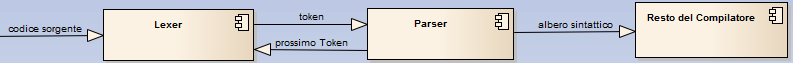
\includegraphics[height=40pt,width=420pt,scale=0.1]{parser.png}}
	\caption{\textit{Posizione del parser all'interno del compilatore.}}
\end{figure}
I metodi di parsing più comunemente utilizzate dai compilatori sono:
\begin{itemize}
	\item \textbf{Parsing top down: }la costruzione dell'albero sintattico avviene partendo dalla radice dell'albero fino ad arrivare alle foglie dell'albero;
	\item \textbf{Parsing bottom up: }la costruzione dell'albero sintattico avviene partendo dalle foglie dell'albero fino ad arrivare alla sua radice.
\end{itemize}
In questa tesi tratteremo il parsing top down in quanto il GLL parsing usa questa metodologia
\section{Grammatiche context-free}
In questo paragrafo introduciamo una notazione - \textit{la grammatica context-free} - utilizzata per specificare la sintassi dei linguaggi di programmazione. Le grammatiche sono usate per descrivere i costrutti dei linguaggi di programmazione. Ad esempio in C, il while può avere la seguente forma:
\begin{align}
	\textbf{while} (espressione) statement \notag
\end{align}
Questa notazione indica che il costrutto è composto dalla parola chiave \textbf{while}, una parentesi tonda aperta, un'espressione, una parentesi tonda chiusa e uno statement. Usando la variabile \textit{expr} che indica una generica espressione e la variabile \textit{stmt} per indicare lo statement, la regola di questo costrutto può essere definita nel seguente modo:
\begin{align}\label{regolaWhile}
	stmt \to \textbf{while } ( exp ) stmt 
\end{align}
in cui la freccia può essere letta come "può avere la forma". Questa regola prende il nome di \textbf{produzione. }All'interno della produzione la parola while, la parentesi aperta e tonda prendono il nome di \textbf{terminali}, mentre le variabili expr e stmt prendono il nome di \textbf{non terminali}.
\subsection{Definizione di grammatica}
Una grammatica context-free è una quadrupla i cui elementi sono \cite{libro: compilatori}:
\begin{enumerate}
	\item \textbf{Terminali. }I terminali sono simboli di base con cui la grammatica definisce il linguaggio. Il termine "\textit{token}" è un sinonimo di terminale.
	\item \textbf{Non-Terminali. }I non-terminali sono variabili sintattiche che denotano un insieme di stringhe. Nella produzione \ref{regolaWhile} \textit{stmt} e \textit{expr} sono non-terminali. Gli insiemi di stringhe rappresentati dai non-terminali concorrono a definire il linguaggio generato dalla grammatica.
	\item \textbf{Simbolo Iniziale. }In una grammatica uno dei non-terminali costituisce il simbolo iniziale e l'insieme di stringhe che esso denota coincide con l'intero linguaggio generato dalla grammatica. 
	\item \textbf{Produzione. }Le produzioni di una grammatica definiscono come i terminali e i non-terminali possono essere combinate a formare stringhe. Ogni produzione è formata da:
	\begin{enumerate}[(a)]
		\item un non-terminale chiamato \textbf{testa}; la produzione definisce alcune delle stringhe denotate alla sua testa;
		\item il simbolo $\to$; a volte il simbolo $\Coloneqq$ è utilizzato al posto della freccia;
		\item un \textbf{ corpo } o \textbf{lato destro} costituito da zero o più non-terminali o terminali; i componenti descrivono un modo in cui le stringhe denotate dal non-terminale della testa possono essere costruite.
	\end{enumerate}
\end{enumerate}
\subsection{Convenzioni notazionali}
In questo paragrafo vengono definite le convenzioni notazionali delle grammatiche che verranno usate nel resto della tesi.
\begin{enumerate}
	\item I seguenti simboli rappresentano i terminali:
	\begin{enumerate}[(a)]
		\item le singole lettere minuscole dell'alfabeto;
		\item i simboli degli operatori matematici e di punteggiatura;
		\item le stringhe minuscole in grassetto;
		\item le cifre numeriche.
	\end{enumerate}
	\item I seguenti simboli sono non-terminali:
	\begin{enumerate}[(a)]
		\item le singole lettere maiuscole dell'alfabeto;  
		\item se usate per descrivere i singoli costrutti della programmazione, le lettere maiuscole possono indicare i non-terminali del linguaggio.
	\end{enumerate}
	\item La testa della prima produzione è il simbolo iniziale.
	\item Un insieme di produzioni del tipo \textit{A$\to$$\alpha_{1}$}, \textit{A$\to$$\alpha_{2}$}, \dots, \textit{A$\to$$\alpha_{k}$}, con una testa comune \textit{A} (che chiamiamo \textit{A-produzioni}), 
	possono essere scritte nel seguente modo: \textit{A}$\to$$\alpha_{1}$ 
	$\mid$ $\alpha_{1}$ $\mid$ $\alpha_{2}$ \dots $\alpha_{k}$. Chiamiamo $\alpha_{1}$, $\alpha_{2}$, \dots , $\alpha_{k}$ le \textit{alternative per A}.
\end{enumerate} 
\subsection{Derivazioni}
Un albero di parsing \cite{libro: compilatori} può essere costruito mediante varie fasi di derivazioni dove, partendo dal simbolo iniziale, ad ogni passo di riscrittura un simbolo non-terminale viene sostituito con il corpo della sua produzione. Tale visione \textit{derivazionale }corrisponde al metodo di costruzione top-down degli alberi di parsing.
Facciamo un esempio. Consideriamo la seguente grammatica:
\begin{align}\label{grammaticaEspressioni}
	E \to E + E \mid E * E \mid - E \mid ( E ) \mid \textbf{id}
\end{align}
La produzione E $\to$ E + E significa che se E indica un'espressione alla anche E + E è un'espressione. La sostituzione di una singola E con E + E si indica con la seguente notazione:
\begin{align}\label{derivazione1}
	E \Rightarrow E + E \Rightarrow \textbf{id} + E \Rightarrow \textbf{id} + \textbf{id}
\end{align}
che si legge "\textit{E} deriva \textit{E + E}. La produzione \textit{E} $\to$ \textit{E + E} può essere utilizzata per sostituire qualsiasi occorrenza di \textit{E} con \textit{E + E} in una qualsiasi stringa di simboli della grammatica. La sequenza \ref{derivazione1} viene definita come una derivazione della stringa \textbf{id }+ \textbf{id} a partire da \textit{E}. Questa derivazione dimostra che la stringa \textbf{id }+ \textbf{id} è una particolare istanza di un'espressione. Ora diamo una definizione formale di concetto di derivazione. $\ll$ Consideriamo un non-terminale \textit{A} posizionata in mezzo ad una sequenza di simboli grammaticali $\alpha$\textit{A}$\beta$ dove $\alpha$ e $\beta$ sono stringhe arbitrarie di simboli grammaticali. Supponiamo che \textit{A} $\to$ $\gamma$ sia una produzione. In tal caso possiamo scrivere $\alpha$\textit{A}$\beta$ $\Rightarrow$ $\alpha$$\gamma$$\beta$, in cui il simbolo $\Rightarrow$ significa "deriva in un solo passo". Quando abbiamo una sequenza di passi di derivazione del tipo $\alpha_{1}$ $\Rightarrow$ $\alpha_{2}$ $\Rightarrow$ \dots $\Rightarrow$ $\alpha_{n}$ in cui possiamo riscrivere $\alpha_{1}$ come $\alpha_{n}$ diremo $\alpha_{1}$ \textit{deriva }$\alpha_{n}$. Per esprimere che una stringa "deriva in zero o più passi" una nuova stringa utilizziamo il simbolo $\overset{*}{\Rightarrow}$. Quindi, 
\begin{enumerate}
	\item $\alpha$ $\overset{*}{\Rightarrow}$ $\alpha$, per qualsiasi stringa $\alpha$;
	\item  se $\alpha$ $\overset{*}{\Rightarrow}$ $\beta$ e $\beta$ $\Rightarrow$ $\gamma$, allora $\alpha$ $\overset{*}{\Rightarrow}$ $\gamma$.
\end{enumerate} 
Inoltre il simbolo $\overset{+}{\Rightarrow}$ significa "deriva in uno o più passi. \par
Se \textit{S} $\overset{+}{\Rightarrow}$ $\alpha$, dove \textit{S} è il simbolo iniziale della grammatica \textit{G}, diciamo che $\alpha$ è una \textbf{forma sentenziale}  di \textit{G}. Una forma sentenziale può contenere sia terminali che non terminali e può essere vuota. Una \textbf{sentenza} o \textbf{frase} di \textit{G} è una forma sentenziale che non contiene nessun non-terminale. Il \textbf{linguaggio generato} da una grammatica \textit{G} è l'insieme di tutte le sue frasi. Quindi una stringa di terminali \textit{w} appartiene a \textit{L(G)}, il linguaggio generato da \textit{G}, se e solo se \textit{w} è una frase di \textit{G}, cioè se \textit{S} $\overset{*}{\Rightarrow}$ \textit{w}. Un linguaggio che può essere generato da una grammatica è detto un \textbf{linguaggio libero dal contesto}. Se due grammatiche generano lo stesso linguaggio sono dette \textbf{equivalenti}.$\gg$ La stringa \textbf{id}+\textbf{id} è una frase della grammatica \ref{grammaticaEspressioni} poichè esiste la derivazione \ref{derivazione1}. Le sequenze di derivazioni prevedono che ad ogni vengano fatte due scelte: la prima scelta consiste nello scegliere il non-terinale da sostituire; la seconda scelta consiste nello scegliere una delle produzioni in cui il non-terminale scelto risulta essere la testa della produzione. Infatti nella derivazione \ref{derivazione1} ogni non-terminale è sostituito con il corpo della produzione corrispondente. Ogni non-terminale da sostituire viene selezionato in questo modo:
\begin{enumerate}
	\item nelle \textit{derivazioni sinistre} si sceglie sempre il non-terminale più a sinistra. La derivazione \ref{derivazione1} è una derivazione a sinistra.
	\item  nelle \textit{derivazioni destre} si sceglie sempre il non-terminale più a destra. 
\end{enumerate}
\subsection{Alberi di parsing}
Un \textbf{albero di parsing} è \cite{libro: compilatori} una rappresentazione grafica di una derivazione che non dipende dall'ordine in cui le produzioni sono utilizzate per rimpiazzare i non-terminali. Ogni nodo interno rappresenta l'applicazione di una produzione ed è etichettato con il non-terminale che indica la testa della  produzione. I figli di questo nodo sono etichettati con i simboli che appaiono nel corpo della produzione utilizzata per sostituire il non-terminale. Un esempio di albero di parsing relativo alla stringa \textbf{id }+\textbf{ id} è mostrato nella figura \ref{fig:albero}.
\begin{figure}[hbpb]
	\centering
	\begin{forest}
		[E
		  [E
		  [\textbf{id}]
		  ]
		  [+]
		  [E
		  [\textbf{id}]
		  ]
		]
	\end{forest}
	\caption{\textit{Albero di parsing relativo alla stringa} \textbf{id} + \textbf{id} }\label{fig:albero}
\end{figure}
Le foglie dell'albero di parsing sono etichettate con terminali o non-terminali che, letti da sinistra verso destra formano una forma sentenziale chiamata \textbf{frontiera} dell'albero. Ora tramite un esempio mostreremo come viene costruito un albero sintattico. \par
\begin{figure}[hbpb]
	\centering
	\begin{forest}
		[E
		[E]
		[+]
		[E]
		]
	\end{forest}
	$\Rightarrow$    
	\begin{forest}
		[E
		[E
		[\textbf{id}]
		]
		[+]
		[E]
		]
	\end{forest}
	$\Rightarrow$    
	\begin{forest}
		[E
		[E
		[\textbf{id}]
		]
		[+]
		[E
		[\textbf{id}]
		]
		]
	\end{forest}
	\caption{\textit{Sequenza di alberi di parsing relativi alla derivazione }\ref{derivazione1}}\label{fig:passiAlbero}
\end{figure}
In figura \ref{fig:passiAlbero} viene rappresentata la sequenza di alberi sintattici costruiti dalla derivazione \ref{derivazione1}. Il primo passo della derivazione \textit{E} $\Rightarrow$ \textit{E} + \textit{E} prevede di aggiungere come radice dell'albero sintattico il simbolo iniziale \textit{E} e come figli \textit{E}, +, ed \textit{E} che corrisponde al corpo della produzione \textit{E} + \textit{E}. Al secondo passo della derivazione \textit{E} $\Rightarrow$ \textbf{id} + \textit{E} aggiungiamo al nodo più a sinistra \textit{E} il nodo figlio \textbf{id}. Così facendo otteniamo al terzo passo il corrispondente albero sintattico per la stringa \textbf{id} + \textbf{id}.
\subsection{Ambiguità}
Una grammatica viene definita \textbf{ambigua} se produce più di un albero sintattico. In altre parole una grammatica ambigua presenta \cite{libro: compilatori} più di una derivazione destra o sinistra per una frase. Facciamo un esempio. Prendiamo in considerazione la grammatica \ref{grammaticaEspressioni} e la frase \textbf{id}+\textbf{id}*\textbf{id}; questa frase presenta due alberi di parsing che sono:\par
\begin{figure}[hbpb]\label{alberibis}
	\centering
	\begin{forest}
		[E
		[E[\textbf{id}]]
		[+]
		[E
		[E[\textbf{id}]] [*][E[\textbf{id}]]]
		]
	\end{forest}
	\begin{forest}
		[E
		[E [E[\textbf{id}]] [+][E[\textbf{id}]]]
		[*]
		[E[\textbf{id}]]
		]
	\end{forest}
	\caption{\textit{Alberi di parsing relativi alla stringa } \textbf{id}+\textbf{id}*\textbf{id}}
\end{figure}
Di conseguenza ciò dimostra che la grammatica \ref{grammaticaEspressioni} risulta essere ambigua.
\subsection{Ricorsione a sinistra}\label{par:ric}
Una grammatica viene definita \textbf{ricorsiva a sinistra} \cite{libro: compilatori} se ha un non-terminale \textit{A} per cui esiste una derivazione \textit{A}$\overset{+}{\Rightarrow}$ \textit{A}$\alpha$ della stringa $\alpha$. Un esempio di ricorsione a sinistra è la seguente produzione:
\[
	term \to term + fact
\]
Le grammatiche ricorsive a sinistre risultano essere problematiche da gestire da parser a discesa ricorsiva perchè entrano in un ciclo infinito. Supponiamo che la procedura per il simbolo \textit{expr} decide di applicare questa produzione. Il corpo inizia con \textit{expr} per cui la procedura per \textit{expr} viene invocata ricorsivamente. Poichè il simbolo di lookahead cambia solo quando si verifica una corrispondenza con un terminale del corpo della produzione, nulla cambia sulla stringa in ingresso che si sta analizzando. Di conseguenza la procedura \textit{expr()} viene chiamata di nuovo e così fino all'infinito.
\section{Parsing top down}
Il parsing top down è una tecnica che prevede di costruire l'albero di parsing per una determinata stringa partendo dalla radice dell'albero fino ad arrivare alle foglie che rappresentano i simmboli della stringa. Questo parsing effettua derivazioni a sinistra sulle stringhe che analizza. Infatti ad ogni passo di computazione il parsing top down cerca di trovare un possibile corpo di produzione da sostituire ad ogni non-terminale. Una volta fatto ciò cerca di trovare una corrispondenza tra i simboli della stringa in ingresso e tra i simboli del corpo della produzione. In questo paragrafo analizzeremo i principi e gli strumenti che usa il parsing top down. Verrà presentato il parsing a discesa ricorsiva che richiede \textit{backtracking} per trovare la produzione opportuna da applicare al non-terminale. Successivamente introdurremo le funzioni FIRST e FOLLOW utilizzate per scegliere la produzione da applicare in base al simbolo in input che si sta analizzando. Poi parleremo delle grammatiche LL(1) ed infine dei parser predittivi che usano le funzioni FIRST e FOLLOW per scegliere le produzioni da sostituire.
\subsection{Parsing a discesa ricorsiva}
Un parsing a discesa ricorsiva è un programma che contiene una procedura per ogni non-terminale della grammatica. L'esecuzione \cite{libro: compilatori} inizia con la procedura relativa al simbolo iniziale e termina con successo se il suo corpo scandisce tutta la stringa d'ingresso. Una procedura per un terminale viene mostrato nella figura 2.5.
\begin{figure}[hbpb]
	%\flushleft
	1) \textbf{void} \textit{A}()$\{$\par
	2)\hspace{0.5cm}Scegli, per \textit{A}, una produzione \textit{A} $\to$ $X_1$, $X_2$ \dots $X_k$;\par
	3)\hspace{0.5cm}\textbf{for}(\textit{i} da 1 fino a \textit{k})$\{$\par
	4)\hspace{1.1cm}\textbf{if}($X_i$ è non-terminale)$\{$\par
	5)\hspace{1.4cm}richiama la procedura $X_i$();\par
	6)\hspace{1.1cm}$\}$\par		
	7)\hspace{1.1cm}\textbf{else}$\{$\par	
	8)\hspace{1.3cm}\textbf{if}($X_i$ è uguale al simbolo d'ingresso corrente a)$\{$\par
	9)\hspace{2.0cm}procedi al simbolo successivo nella sequenza d'ingresso;\par
   10)\hspace{1.3cm}$\}$\par
   11)\hspace{1.4cm}\textbf{else}$\{$/* si è verificato un errore */;$\}$\par
   12)\hspace{0.5cm}$\}$\par
   13) $\}$\par
	\caption{\textit{Procedura di un non-terminale per un parser top down}}\label{fig:code}
\end{figure}

Lo pseudocodice mostrato \cite{libro: compilatori} in questa figura è non-deterministico poichè inizia con la scelta di quale produzione utilizzare per \textit{A} senza indicare come deve essere fatta la scelta. Questo metodo può richiedere backtracking, cioè può richiedere di rileggere più di una volta la stringa in ingresso. Per aggiungere il backtracking al codice in figura \ref{fig:code}. La linea (2) va tolta e rimpiazzata con istruzioni in cui $\ll$ è necessario provare ognuna delle possibili produzioni secondo un certo ordine. In questo caso il fallimento alla linea (11) non è un fallimento "definitivo", ma indica una necessita di tornare alla linea (2) e provare un'altra produzione. Solo se non vi sono più produzioni per \textit{A} da provare si segnala che è stato identificato un errore nella stringa d'ingresso. Quindi se vogliamo provare una nuova produzione per \textit{A}, a seguito di un fallimento, dobbiamo essere in grado di riportare il puntatore alla stringa d'ingresso alla posizione in cui si trovava quando abbiamo raggiunto la linea (2) per la prima volta. $\gg$ Una grammatica ricorsiva a sinistra risulta essere compromettente per questo tipo di parser in quanto può entrare in un ciclo infinito. Per maggiori dettagli si veda il paragrafo \ref{par:ric}
\subsection{Funzioni FIRST e FOLLOW}
Per stabilire quale produzione applicare per sostituire un non-terminale basandoci sui simboli della stringa in input, i parser, sia quelli top-down e bottom-up, usano le funzione FIRST e FOLLOW.\par
Definiamo \textbf{FIRST}($\alpha$), \cite{libro: compilatori} in cui $\alpha$ è una generica stringa di simboli della grammatica, come l'insieme dei terminali che costituiscono l'inizio delle stringhe derivabili da $\alpha$. Se $\alpha$ $\overset{*}{\Rightarrow}$ $\epsilon$, allora anche $\epsilon$ appartiene all'insieme FIRST.\par
Definiamo \textbf{FOLLOW}(\textit{A}), in cui \textit{A} è un non-terminale, come l'insieme dei simboli terminali che possono apparire immediatamente alla destra di \textit{A}in qualche forma sentenziale, cioè l'insieme dei terminali \textit{a} per cui esiste una derivazione nella forma \textit{A} $\overset{*}{\Rightarrow}$ $\alpha$\textit{Aa}$\beta$, dove $\alpha$ e $\beta$ sono generiche forme sentenziali. Se \textit{A} appare come simbolo più a destra di una forma sentenziale, allora $\$$ appartiene al FOLLOW(\textit{A}).
\begin{enumerate}
	\item Se \textit{X} è non terminale, FIRST(\textit{X}) = $\{$.
	\item Se \textit{X} è un non-terminale ed esiste una produzione del tipo \textit{X} $\to$ $Y_1$$Y_2$\dots$Y_k$ con \textit{k}$\geq$1, allora si aggiunga \textit{a} a FIRST(\textit{X}) se per qualche valore di \textit{i}, \textit{a} appartiene a FIRST(\textit{$Y_i$}) e $\epsilon$ appartiene a tutti gli insiemi FIRST(\textit{$Y_1$}), \dots, FIRST(\textit{$Y_{i-1}$}), cioè se $Y_1$ \dots $Y_{i-1}$ $\overset{*}{\Rightarrow}$ $\epsilon$. Se $\epsilon$ appartiene a FIRST(\textit{$Y_j$}) per \textit{j} = 1,2,\dots,\textit{k}, allora si aggiunga $\epsilon$ all'insieme FIRST(\textit{X}); se invece $Y_1$ $\overset{*}{\Rightarrow}$ $\epsilon$si aggiunga FIRST(\textit{$Y_2$}) a FIRST(\textit{X}), e così via.
	\item Se esiste una produzione \textit{X} $\to$ $\epsilon$, si aggiunga $\epsilon$ a FIRST(\textit{X}). 
\end{enumerate}
Per calcolare FOLLOW(\textit{A}) per tutti i non-terminali \textit{A} si usano le seguenti regole:
\begin{enumerate}
	\item Si aggiunga $\$$ a FOLLOW(\textit{S}), ricordando che \textit{S} è il simbolo iniziale e $\$$ è il marcatore di fine della stringa d'ingresso;
	\item Se esiste una produzione del tipo A $\to$ $\alpha$\textit{B}$\beta$, allora si aggiunga a FOLLOW(\textit{B}) ogni elemento di FIRST($\beta$) eccetto $\epsilon$.
	\item Se esiste una produzione del tipo \textit{A} $\to$ $\alpha$\textit{B} oppure del tipo \textit{A} $\to$ $\alpha$\textit{B}$\beta$ per cui FIRST($\beta$) contiene $\epsilon$, allora tutti i simboli in FOLLOW(\textit{A}) appartengono a FOLLOW(\textit{B}) $\gg$
\end{enumerate}
Facciamo un esempio di come si calcolano FIRST e FOLLOW su una grammatica. Consideriamo la seguente grammatica:
\begin{align}\label{grammatica2}
	I  & \to A \notag \\
	A  & \to S \notag \\ 
	S  & \to CC \notag \\
	C  & \to cC \mid d 
\end{align}
I FIRST e FOLLOW di questa grammatica sono:
\begin{enumerate}
	\item FIRST(\textit{I})=FIRST(\textit{A})=FIRST(\textit{S})=FIRST(\textit{C})=$\{$c,d$\}$. Per capire il motivo di ciò, si noti che le due produzioni per \textit{C} hanno i corpi che iniziano con i due simboli terminali c e d. Poichè \textit{S}, ha solo una produzione che inizia per \textit{C} e non deriva $\epsilon$, il FIRST(\textit{S}) coincide con FIRST(\textit{C}). Lo stesso ragionamento lo si può applicare per FIRST(\textit{S}) e FIRST(\textit{A})
	\item FOLLOW(\textit{I})=FOLLOW(\textit{A})=FOLLOW(\textit{S})=$\{$$\$$$\}$. Dato che \textit{I} è il simbolo iniziale, il FOLLOW(\textit{I}) deve contenere il carattere speciale $\$$. Poichè \textit{S} e \textit{A} appaiono da sole nel corpo di altre produzioni nè consegue che sono seguite dal simbolo di fine stringa $\$$. Pertanto il  FOLLOW(\textit{A}) e  FOLLOW(\textit{S}) coincide con il  FOLLOW(\textit{I}).
	\item FOLLOW(\textit{C})=$\{$c,d,$\$$$\}$. All'interno di una produzione il simbolo \textit{C} è seguito da un altro simbolo \textit{C}. Pertanto il FOLLOW(\textit{C}) include i simboli del FIRST(\textit{C}). Inoltre essendo che il simbolo \textit{C} risulta essere l'ultimo simbolo all'interno di una produzione allora il simbolo $\$$ rientra nel FOLLOW(\textit{C}).
\end{enumerate}
\subsection{Grammatiche LL(1)}
Un parser predittivo viene sempre costruito a partire da una grammatica della classe LL(1). La prima L \cite{libro: compilatori} indica che la stringa in input che si sta analizando viene letta da sinistra verso destra. La seconda L specifica che viene fatta una derivazione a sinistra; infine l'1 fra le parentesi indica che le decisioni del parser vengono fatte analizzando un solo simbolo di lookhead. Data una grammatica G con due produzioni \textit{A} $\to$ $\alpha$ $\mid$ $\beta$ è definita LL(1) se sono verificate le seguenti condizioni: $\ll$
\begin{enumerate}
	\item non esiste alcun terminale \textit{a} tale che sia $\alpha$ sia $\beta$ derivano stringhe che iniziano con \textit{a};
	\item al più una tra $\alpha$ e $\beta$ deriva la stringa nulla $\epsilon$;
	\item se $\beta$ $\overset{*}{\Rightarrow}$ $\epsilon$ non deriva alcuna stringa che inizia con un non terminale appartenente all'inisieme FOLLOW(\textit{A}); allo stesso modo, se $\alpha$ $\overset{*}{\Rightarrow}$ $\epsilon$, allora  $\beta$ non deriva alcuna stringa che inizia con un terminale in FOLLOW(\textit{A}). $\gg$
\end{enumerate}
Le prime due condizioni verificano che FIRST($\alpha$) e FIRST($\beta$) sono insiemi disgiunti. La terza condizione verifica che se $\epsilon$ appartiene a FIRST($\beta$) allora FIRST($\alpha$) e FOLLOW(\textit{A}) sono insiemi disgiunti; la stessa cosa vale se $\epsilon$ appartiene a FIRST($\alpha$). Quindi in base a ciò un parser predittivo per una grammatica LL(1) può essere sempre costruito se ad ogni passo di computazione posso sostituire un non-terminale con una sola produzione che viene scelta in base al simbolo di input corrente. Ovviamente nessuna grammatica ambigua e ricorsiva a sinistra può essere una grammatica LL(1). L'algoritmo seguente raccoglie le informazioni di FIRST e FOLLOW in una \textbf{tabella di parsing predittivo}, cioè una matrice bidimensionale \textit{M}[\textit{A},\textit{a}] dove \textit{A} è un non-terminale e \textit{a} è un terminale oppure il simbolo $\$$. L'algoritmo sceglie la produzione \textit{A} $\to$ $\alpha$ solo se il simbolo in input \textit{a} appartiene a FIRST($\alpha$). Quando invece abbiamo a che fare con derivazioni \textit{a} $\overset{*}{\Rightarrow}$ $\epsilon$, scegliamo sempre la produzione \textit{A} $\to$ $\alpha$ se il simbolo corrente appartiene al FOLLOW(\textit{A}) o si è raggiunto il simbolo $\$$ nella stringa in input e se tale simbolo appartiene a FOLLOW(\textit{A}).\par
\textbf{\underline{Algoritmo 1}} Cotruzione di una tabella di parsing predittivo.\par 
\vspace{0.2cm}\textbf{INPUT} Una grammatica \textit{G}.\par
\textbf{OUTPUT} Una tabella di parsing M.\par 
\textbf{METODO} Per ogni produzione \textit{A} $\to$ $\alpha$ della grammatica \textit{G} si svolgano i seguenti passi.
\begin{enumerate}
	\item Per ogni terminale \textit{a} in FIRST($\alpha$) si aggiunga \textit{A} $\to$ $\alpha$ a \textit{M}[\textit{A},\textit{a}].
	\item Se $\epsilon$ appartiene a FIRST($\alpha$), allora per ogni terminale \textit{b} FOLLOW(\textit{A}) si aggiunga \textit{A} $\to$ $\alpha$ a \textit{M}[\textit{A},\textit{b}]. Se $\epsilon$ appartiene a FIRST($\alpha$) e $\$$ a FOLLOW(\textit{A}), si aggiunga \textit{A} $\to$ $\alpha$ anche a \textit{M}[\textit{A},$\$$].
\end{enumerate}
Se dopo questi passi non vi è alcuna produzione in \textit{M}[\textit{A},\textit{a}], si ha una condizione di errore, che viene indicata vuota nella casella corrispondente.\\ 
Facciamo un esempio e prendiamo in riferimento grammatica \ref{grammatica2}. Applichiamo l'algoritmo precedente ed otteniamo la seguente tabella di parsing.
\begin{table}[hbpb]
	\centering
	\label{tabellaparsing}
	\begin{tabular}{ccccc} %\hline 
		\toprule
		%\multirow{2}*{\textbf{Non Terminale}} & %\multicolumn{4}{c}{\textbf{Simbolo d'ingresso}} \\ 
		%\cmidrule(lr){2-4}
		& c & d & $\$$ \\ 
		\midrule
		\textit{I}			& \textit{I} $\to$ \textit{A}  & \textit{I} $\to$ \textit{A} &    \\ 
		\textit{A} 			& \textit{A} $\to$ \textit{S}  & \textit{A} $\to$ \textit{S} &    \\ 
		\textit{S}			& \textit{S} $\to$ \textit{CC} & \textit{S} $\to$ \textit{CC} &   \\ 
		\textit{C} 			& \textit{C} $\to$ \textit{cC}& \textit{C} $\to$ \textit{d} &     \\ 
		\bottomrule
	\end{tabular}
	\caption{\textit{Tabella di parsing della grammatica }\ref{grammatica2}}
\end{table} \par
Gli spazi bianchi indicano una condizione d'errore, mentre gli altri indicano quale produzione usare per sostituire un non-terminale in base ad un determinato simbolo in input. Si consideri, per esempio la produzione \textit{I} $\to$ \textit{A}. Dato che FIRST(\textit{A}) = FIRST(\textit{S}) questa produzione viene aggiunta sia {\textit{M}[\textit{A},\textit{c}] e a {\textit{M}[\textit{A},\textit{d}].
\subsection{Parsing predittivo non ricorsivo}
Un parser predittivo non ricorsivo \cite{libro: compilatori} viene costruito usando uno stack, piuttosto che effettuare le chiamate ricorsive. Se \textit{w} è la porzione dell'ingresso riconosciuta a un certo momento, allora lo stack contiene una sequenza di simboli grammaticali $\alpha$ tali che \textit{S} $\overset{*}{\Rightarrow}$ \textit{w}$\alpha$. Questo parser usa un buffer d'ingresso,che contiene anche il simbolo $\$$ per segnare la fine della stringa, uno stack che contiene i simboli grammaticali e la tabella di parsing costrtuita mediante l'algoritmo 1. Il fondo dello stack viene segnalato con il simbolo $\$$. Il parser funziona nel seguente modo:
\begin{enumerate}
	\item riceve in input una stringa \textit{w} e una tabella di parsing \textit{M} relativa a una grammatica \textit{G};
	\item \label{PASSO} ad ogni passo di computazione controlla il simbolo \textit{X} in cima allo stack e un simbolo \textit{a} della stringa \textit{w} in input.
	\item Se \textit{X} è un non-terminale, il parser lo sostituisce con il corpo della produzione che si trova nella posizione \textit{M}[\textit{X},\textit{a}];
	\item Altrimenti, se \textit{X} è un terminale, allora il parser verifica la corrispondenza di \textit{X} con il simbolo \textit{a} e se esiste legge il simbolo successivo della stringa \textit{w}.
	\item Ripetere il passo \ref{PASSO}.
	\item Il parser termina con sucesso se lo stack non contiene nessun simbolo \textit{X} e ciò determina che la stringa letta fa parte della grammatica \textit{G}.
\end{enumerate}
Di seguito vengono riportate le mosse del parser predittivo applicate alla grammatica \ref{grammatica2}.
\begin{table}[hbpb]
	\centering
	\label{tabellaStack}
	\begin{tabular}{cclc}
		\toprule
		\textbf{Input} & \textbf{Stack} & \textbf{Azione} & \textbf{Riconosciuta}\\
		\midrule
		\textbf{cdd$\$$} & \textit{I$\$$}  \\
		\textbf{cdd$\$$} & \textit{A$\$$}  & output \textit{I} $\to$ \textit{A} \\
		\textbf{cdd$\$$} & \textit{S$\$$}  & output \textit{A} $\to$ \textit{S} \\
		\textbf{cdd$\$$} & \textit{CC$\$$}  & output \textit{S} $\to$ \textit{CC} \\
		\textbf{cdd$\$$} & \textit{cCC$\$$}  & output \textit{C} $\to$ \textit{cC} \\
		\textbf{dd$\$$} & \textit{CC$\$$}  & consuma \textbf{c} & \textbf{c}\\
		\textbf{dd$\$$} & \textit{dC$\$$}  & output \textit{C} $\to$ \textit{d} & \textbf{c}\\
		\textbf{d$\$$} & \textit{C$\$$}  & consuma \textbf{d} & \textbf{cd}\\
		\textbf{d$\$$} & \textit{d$\$$}  & output \textit{C} $\to$ \textit{d} & \textbf{cd}\\
		\textbf{$\$$} & \textit{$\$$}  & consuma \textbf{d} & \textbf{cdd}\\
		\bottomrule
	\end{tabular}
	\caption{\textit{Mosse di un parser predittivo sulla stringa \textbf{cdd}} }
\end{table}\\
In questa tabella la cima dello stack è riportata a sinistra nella colonna "Stack". Tali mosse corrispondono alla derivazione sinistra; infatti abbiamo che:
\begin{align}
	I \Rightarrow A \Rightarrow S \Rightarrow CC \Rightarrow cCC \Rightarrow cdC \Rightarrow cdd \notag
\end{align}
Si noti che le forme sentenziali in tale derivazione corrispondono alla porzione di stringa in input già analizzata (indicata nella colonna riconosciuta).
\section{Conclusioni}
In questo capitolo è stato discusso di come funziona il parsing top down ed in particolare si è discusso degli algoritmi di parsing LL(1). Questo parser, però, presenta dei limiti:
\begin{itemize}
	\item Non sono adatti per grammatiche ambigue e ricorsive a sinistre;
	\item Non ammettono tabelle di parsing in cui vi sono più produzioni per un simbolo d'ingresso.
\end{itemize}
Delle possibili soluzioni a questi limiti prevedono: eliminazione dell'ambiguità e della ricorsione a sinistra dalla grammatica, l'uso della fattorizzazione a sinistra per rendere la grammatica più adatta al parsing predittivo o l'uso di parsing generalizzati top down che usano il non-determinismo per superare i conflitti che trova un parser predittivo nelle tabelle di parsing. Nel capitolo successivo discuteremo di quest'ultima soluzione.